\begin{frame}{Marking \underline{global} inconsistencies}
  Consider this program:
  \[%
    \ELam{f}{\TUnknown}{\EAp{f}{(\EPlus{f}{1})}}
  \]%

  \pause
  $\assignType{f}{\TUnknown}$, so the bidirectional system operates gradually, \pause
  but $f$ is 
  %
  \pause
  \begin{enumerate}
    \item applied as a function \pause (a function?)
      \pause
    \item an operand of $\ECOpPlus$ \pause (a number?)
  \end{enumerate}

  \pause
  \vspace{1em}
  \emph{Global, constraint-based type checking would have caught this!}
\end{frame}

\begin{frame}{Layers upon layers}
  Get the best of both worlds by layering \textbf{constraint-based inference} 
  atop the marked lambda calculus

  \vspace{1em}
  \pause
  \begin{itemize}
    \item The marked lambda calculus localizes and recovers predictably from \emph{local inconsistencies}

      \pause
    \item \textbf{Type hole inference} solves and marks \emph{global inconsistencies}

      \pause
      \begin{itemize}
        \item Not meant to be a standalone type checker
        \item Downstream service to supplement the marked lambda calculus
      \end{itemize}
  \end{itemize}
\end{frame}

\newcommand{\Id}[1]{\ensuremath{\goodcolor{hole}{#1}}}
\newcommand{\IdU}{\ensuremath{\Id{u}}}
\newcommand{\ProvU}{\ensuremath{\IdU}}
\newcommand{\ProvExp}[1]{\ensuremath{exp\goodcolor{\colorOkSideJudge}{(}#1\goodcolor{\colorOkSideJudge}{)}}}
\newcommand{\ProvIn}[1]{\ensuremath{\to_L\goodcolor{\colorOkSideJudge}{(}#1\goodcolor{\colorOkSideJudge}{)}}}
\newcommand{\ProvOut}[1]{\ensuremath{\to_R\goodcolor{\colorOkSideJudge}{(}#1\goodcolor{\colorOkSideJudge}{)}}}
\newcommand{\PTS}{\operatorname{\mathsf{PotentialTypeSet}}}
\newcommand{\cursor}{\ensuremath{\goodcolor{\colorOkSideJudge}{\bm{\wedge}}}}

\begin{frame}{Type hole inference}
  \begin{itemize}
    \item Occurrences of $\TUnknown$ arise from
      \pause (1) \emph{type holes}, \eg, in $\ELam{x}{\TUnknown}{\cdots}$ \\
      \pause or (2) error marks

      \pause
    \item Gather constraints from the bidirectional system\pause,
      treating occurrences of $\TUnknown$ as unification variables
      {\footnotesize\parencite{siek2008}}

      \pause
    \item Solve them via a standard unification algorithm {\footnotesize\parencite{huet1976}} \\
      \pause whilst accumulating all $\PTS(\TUnknown^{\Provp})$
      %
      \pause
      \begin{itemize}
        \item Set of all potential type \emph{fillings}, inferred from constraints
          \pause
        \item To unify $\constrain{\TMV_1}{\TMV_2}$, recursively merge
          $\mathsf{PotentialTypeSet(\TMV_1)}$ and $\mathsf{PotentialTypeSet(\TMV_2)}$
      \end{itemize}
  \end{itemize}
\end{frame}

\begin{frame}
  \[%
    \ELam{f}{\TUnknown^{\Id{1}}}{\EAp{f}}{(\EPlus{f}{1})}
  \]%

  \uncover<2->{
    yields the constraints
    \[%
      \{ \onderset<6>{\cursor}{\constrain{\TUnknown^{\Id{1}}}{\TArrow{\TUnknown^{\ProvIn{\Id{1}}}}{\TUnknown^{\ProvOut{\Id{1}}}}}}
       \only<3->{, \onderset<7>{\cursor}{\constrain{\TNum}{\TUnknown^{\Id{1}}}}}
       \only<4->{, \onderset<8>{\cursor}{\constrain{\TNum}{\TUnknown^{\ProvIn{\Id{1}}}}}} \}
    \]%
  }
  
  \vspace{-1em}
  \uncover<5->{
    and solving gives
    \[%
      \PTS(\TUnknown^{\Id{1}})
        =
      \Alt<6->{
        \Alt<7->{
          \Alt<8->{
            \{ \TArrow{\{ \onderline<8>{\TNum} \}}{\{ \TUnknown^{\ProvOut{\Id{1}}} \}},
               \TNum \}
          }{
            \{ \TArrow{\{ \TUnknown^{\ProvIn{\Id{1}}} \}}{\{ \TUnknown^{\ProvOut{\Id{1}}} \}},
             \underline{\TNum} \}
          }
        }{
          \{ \underline{\TArrow{\{ \TUnknown^{\ProvIn{\Id{1}}} \}}{\{ \TUnknown^{\ProvOut{\Id{1}}} \}}} \}
        }
      }{
        \{ \}
      }
    \]%
  }

  \vspace{-1em}
  \onslide<9->{
    Two \emph{potential fillings} of $\TUnknown^{\Id{1}}$ are $\TArrow{\TNum}{\TUnknown}$ and
    $\TNum$\onslide<10->{, which is more than one; inconsistent constraints!}
  }
\end{frame}

\begin{frame}[fragile]
  \begin{center}
    \alt<2->{
      \alt<3->{
        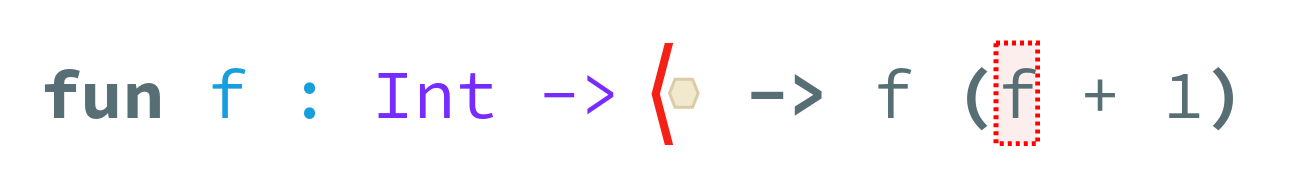
\includegraphics[width=0.9\textwidth]{inference-arrow.png}
      }{
        
\includegraphics[width=0.9\textwidth]{inference-int.png}
      }
    }{
      
\includegraphics[width=0.9\textwidth]{inference.png}
    }
    \vspace{2em}
    \alt<2->{
      \alt<3->{
        
\includegraphics[width=0.9\textwidth]{inspector-arrow.png}
      }{
        
\includegraphics[width=0.9\textwidth]{inspector-int.png}
      }
    }{
      
\includegraphics[width=0.9\textwidth]{inspector.png}
    }
  \end{center}

  Hazel \textcolor{BrickRed}{\small[\href{https://hazel.org}{hazel.org}]}
  offers the user ability to fill either in

  \begin{tikzpicture}[remember picture,overlay]
    \node[xshift=-4.6cm, yshift=-5cm, visible on=<2>] at (current page.north east) { \mousePointer };
    \node[xshift=-2.3cm, yshift=-5cm, visible on=<3>] at (current page.north east) { \mousePointer };
  \end{tikzpicture}
\end{frame}

\begin{frame}
  This approach is \emph{neutral}

  \vspace{1em}
  \pause
  \begin{itemize}
    \item Localize errors to the originating type hole or error mark\pause, \\
      instead of guessing about user intent

      \pause
    \item All potential type hole fillings are provided to the user for selection

      \pause
    \item Control returned to bidirectional system after user selects
  \end{itemize}
\end{frame}
